\documentclass[12pt]{article}

\usepackage{graphicx} % Allows including images
\usepackage{booktabs} % Allows the use of \toprule, \midrule and \bottomrule in tables
\usepackage{amsmath}
\usepackage{amsfonts}
\usepackage{ifthen}
\usepackage{amssymb}
\usepackage{amsbsy}
\usepackage{bm}
\usepackage{ulem}
\usepackage{float}
\usepackage{latexsym}
\usepackage{comment}
\usepackage{graphicx}
\usepackage{amstext}
\usepackage{latexsym}
\usepackage{arydshln}
\usepackage{longtable}
\usepackage{enumerate}
\usepackage{multirow}
\usepackage{cases}
\usepackage{geometry}
\usepackage{mathtools}
\usepackage{subeqnarray}
\usepackage{textcomp}
\usepackage{hyperref}
%\usepackage{subfigure}
\usepackage{url}
\usepackage{threeparttable}
\usepackage{xr}
\usepackage{multirow}
\usepackage{wrapfig}
\usepackage{lscape}
\usepackage{rotating}
\usepackage{subcaption}
\usepackage{epstopdf}
\usepackage{verbatim}
\usepackage{xcolor}
\usepackage[sort&compress]{natbib}
\usepackage{bm}


\captionsetup{font={small}}
\geometry{left=2.0cm, right=2.0cm, top=2.5cm, bottom=2.5cm}

\title{EE526 Homework 4}

\author{Xingche Guo}

\date{\today}

\linespread{1.3}
\begin{document}
\maketitle

%%%%%%%%%%%%%%%%%%%%%%
\section*{Problem 1}

\begin{figure}[h] 
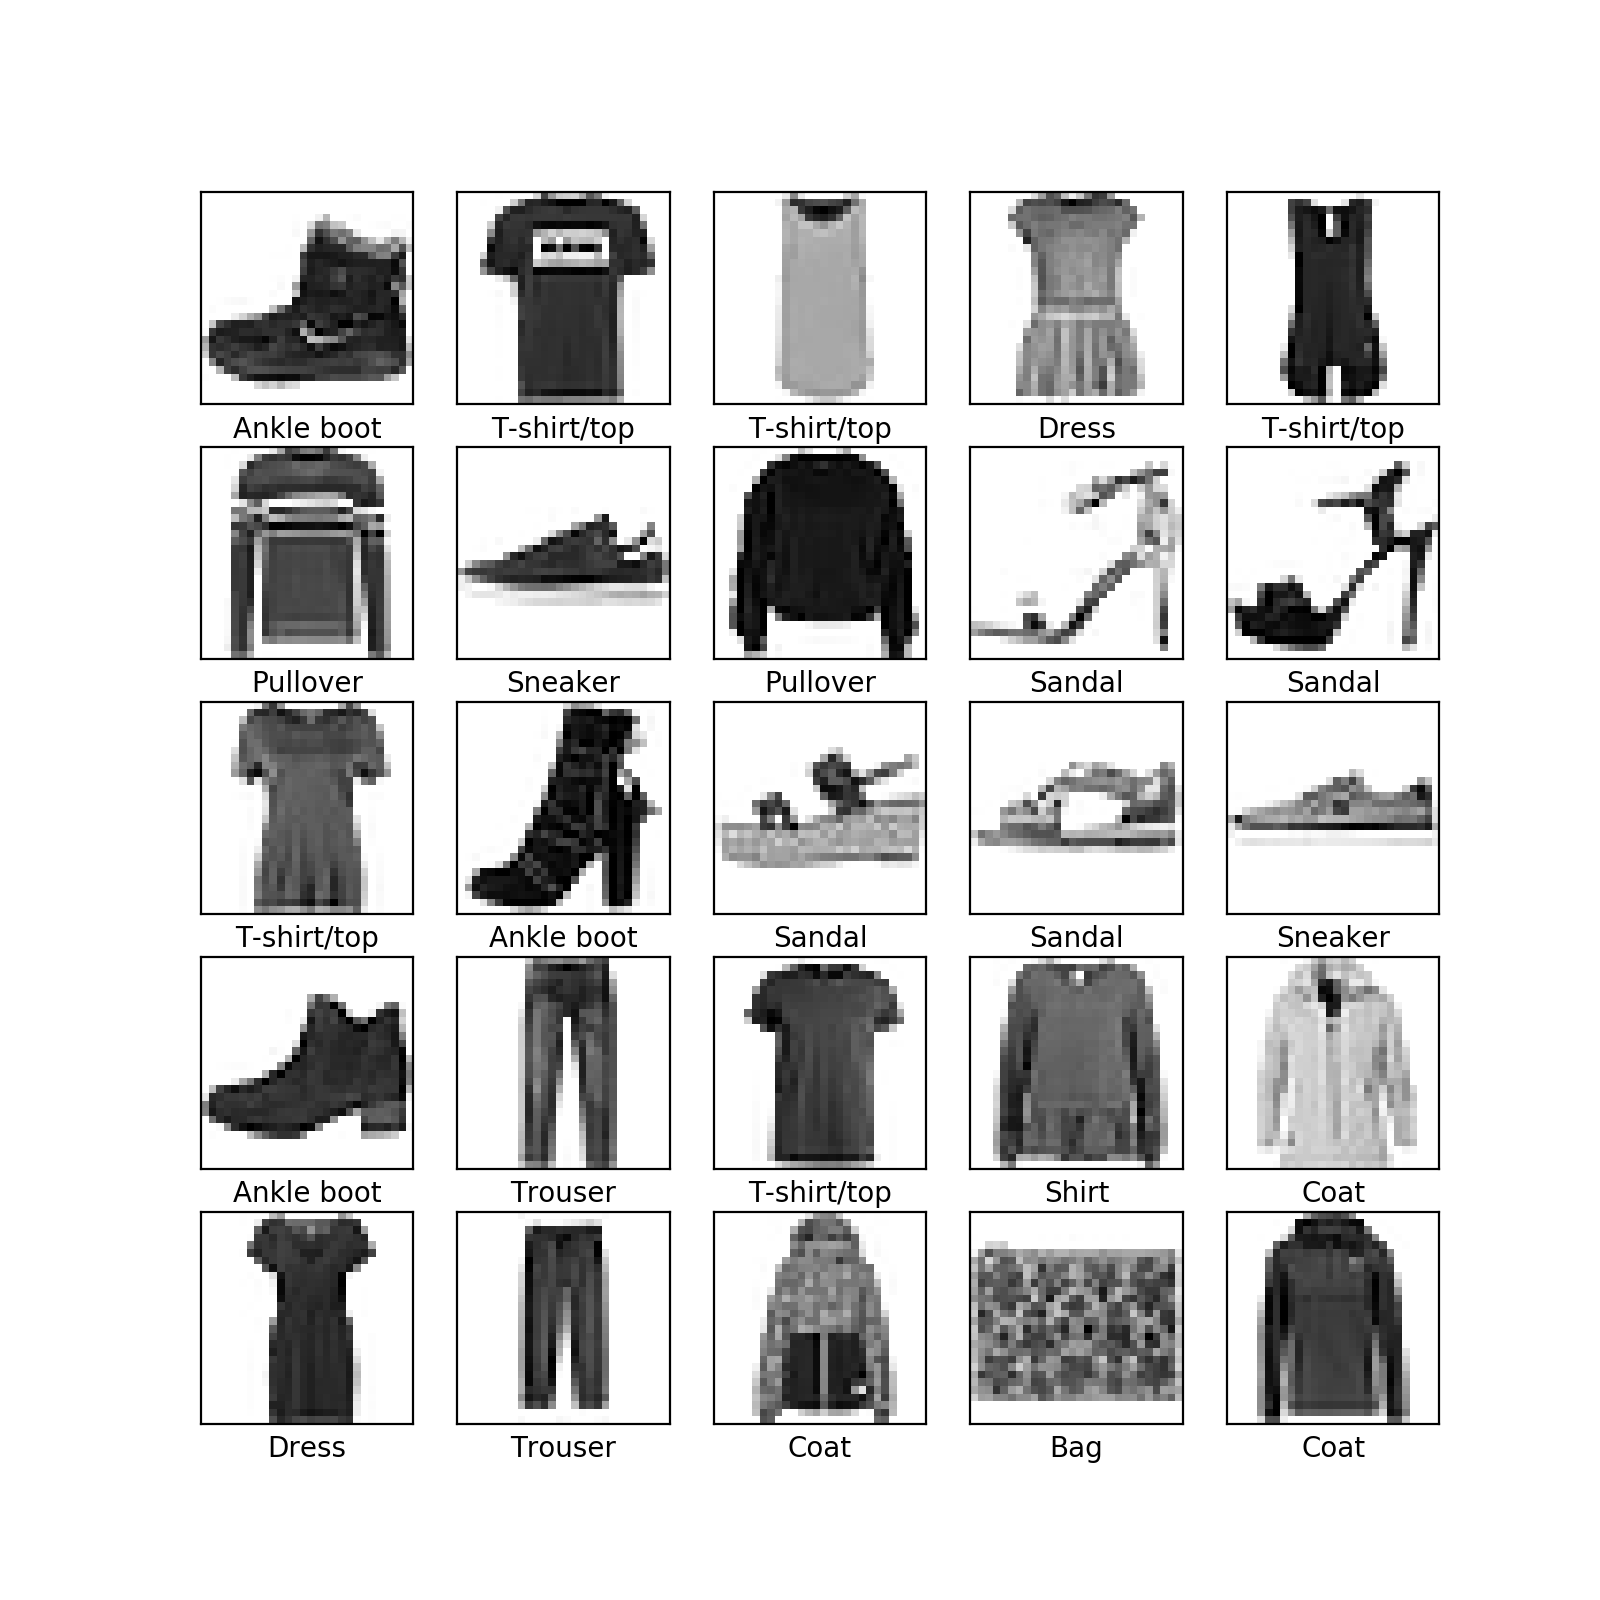
\includegraphics[width=0.65\textwidth]{train_examples.png}
\caption{}
\end{figure}

In this problem, CNN is implemented to the Fashion MNIST classification problem. See the visualization of the training data in Figure 1.


\subsection*{(a)}

\begin{figure}[h] 
\centering
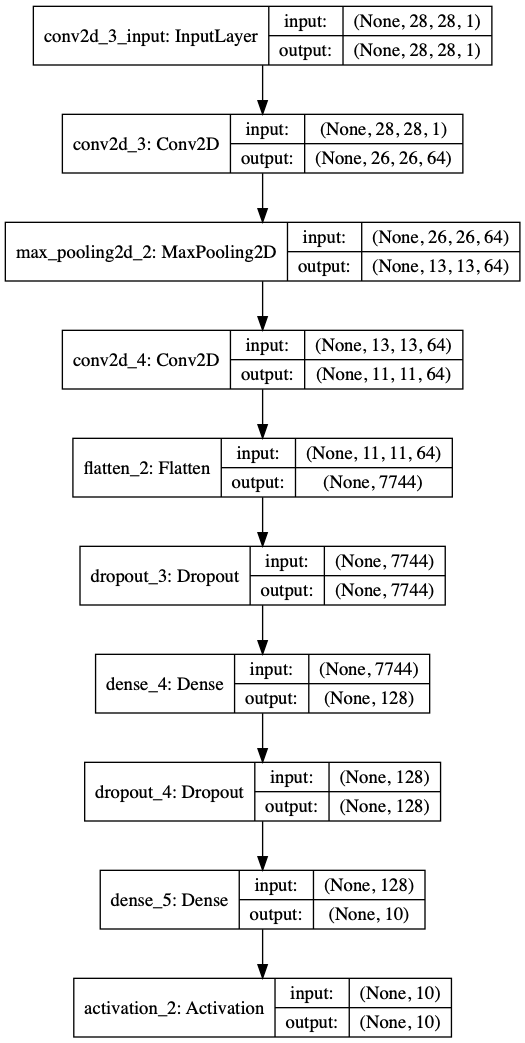
\includegraphics[width=0.4\textwidth]{cnn_model.png}
\caption{}
\end{figure}

The CNN architecture can be found in Figure 2. Specifically, two convolutional layers and two fully connected layers are used. Batch size is chosen to be 128 and a total of 20 epochs are used. There are:
$$
(1 \times 3 \times 3 \times 64 + 64) + (64 \times 3 \times 3 \times 64 + 64) + (7744 \times 128 + 128) + (128 \times 10 + 10) = 640 + 36928  + 991360 + 1290 
$$
parameters used.


\subsection*{(b)}

In each forward pass, a total number of floating point operations needed is:
$$
multiplication: \ \ (3 \times 3 \times 26 \times 26 \times 64) + (3 \times 3 \times 11 \times 11 \times 64) + (7744 \times 128) + (128 \times 10) = 1451584
$$
$$
addition: \ \ [ (8 + 1) \times 26 \times 26 \times 64] + [(8 + 1) \times 11 \times 11 \times 64] + [(7743+1) \times 128] + [(127+1) \times 10] = 1451584
$$
Thus, a total number of floating point operations needed $\approx 3 \times 10^6$.


\subsection*{(c)}

In each mini-batch the total floating point operations needed $\approx 1.5 \times 10^9$.


\subsection*{(d)}

The total floating point operations per epoch needed $\approx 7.2 \times 10^{11}$. The total floating point operations over the whole training process needed $\approx 1.4 \times 10^{13}$.


\subsection*{(e)}

\begin{figure}[h] 
\centering
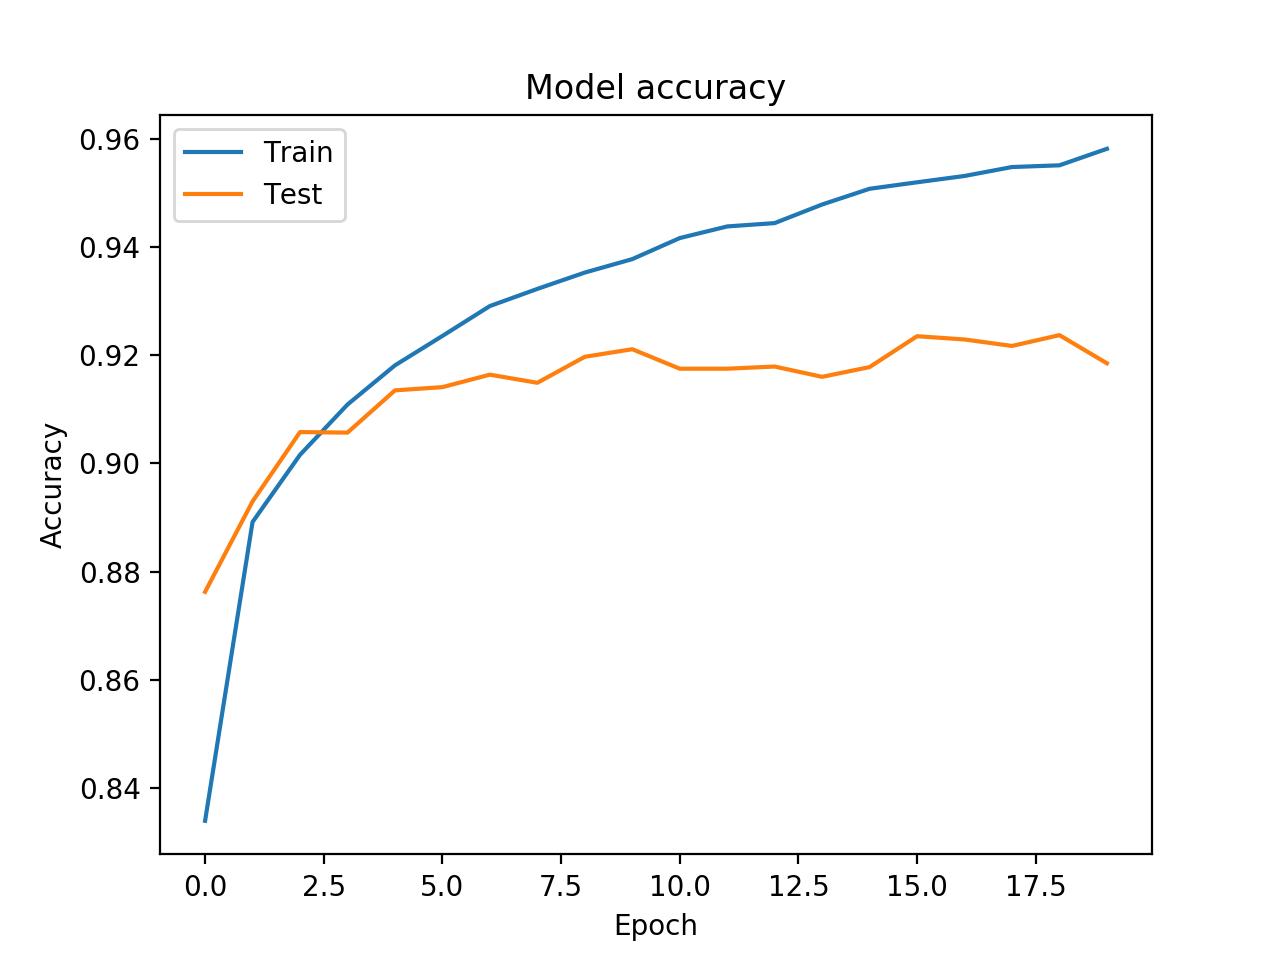
\includegraphics[width=0.7\textwidth]{acc.png}
\caption{}
\end{figure}

Train accuracy: $97.7\%$; Test accuracy: $92.5\%$. A plot of the training accuracy and test accuracy is shown in Figure 3.





%%%%%%%%%%%%%%%%%%%%%%
\section*{Problem 2}

\begin{figure}[h] 
\centering
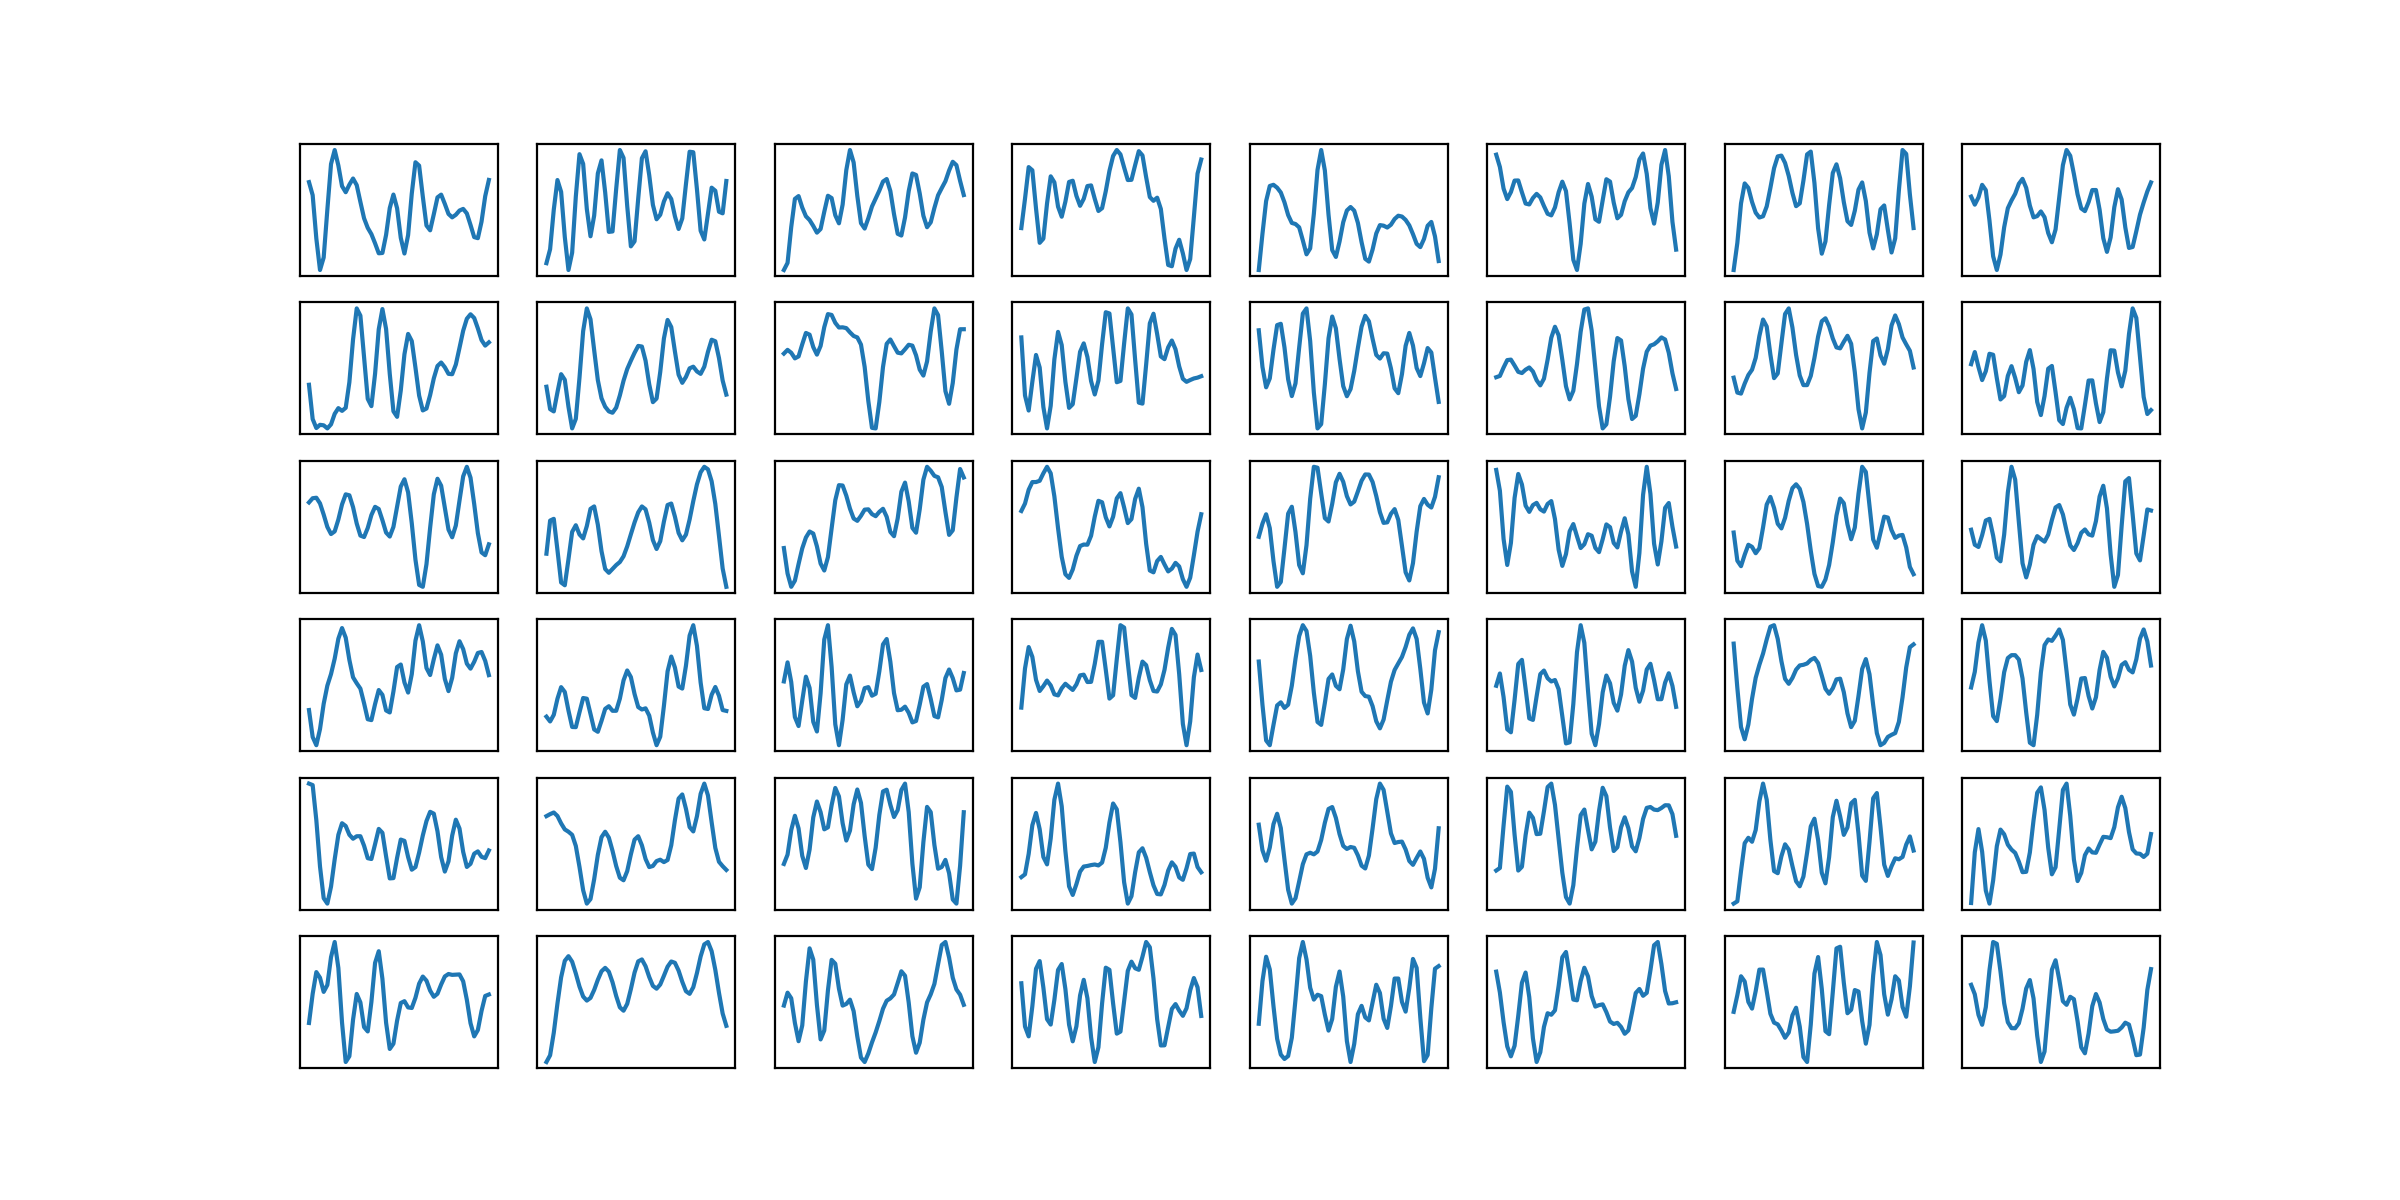
\includegraphics[width=1.0\textwidth]{train_examples2.png}
\caption{}
\end{figure}

In this problem, RNN is implemented to the time series prediction problem. The dataset contains 100 signals (the network should be trained based on the first 66 signals and tested using the last 34 signals), for each signal, there are 500 (equally spaced) measurements. See the visualization of 48 randomly chosen signals (first 50 measurements) in Figure 4. We regard the the $1:499$ measurements as $X$, and the $2:500$ measurements as $Y$, and apply the RNN model with 3 recurrent layers and one final non-recurrent layer, the details can be found in Figure 5. We let the number of epochs to be $5,000$, the training and testing loss for each epochs are plot in Figure 6. We also compared the true $Y_{test}$ to the prediction of $Y_{test}$, the prediction results can be found in Figure 7.

One strange thing is that train loss is larger than the testing loss, I guess the problem is that we do not run enough iterations. I also tried to hold out more time measurements (say, predict the last 5 measurements instead of the last one measurement). However, it requires a more complex model and the RNN will converge much slower.





\begin{figure}[h] 
\centering
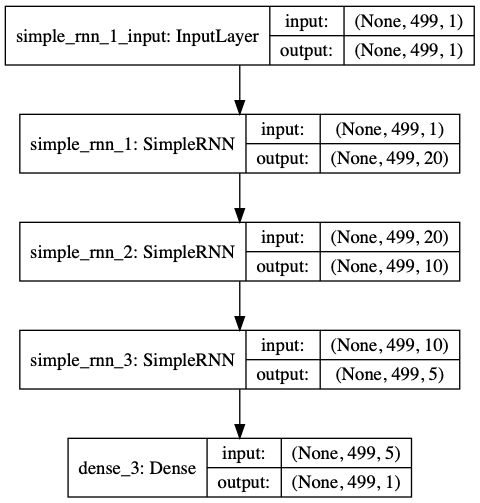
\includegraphics[width=0.5\textwidth]{rnn_model.png}
\caption{}
\end{figure}


\begin{figure}[h] 
\centering
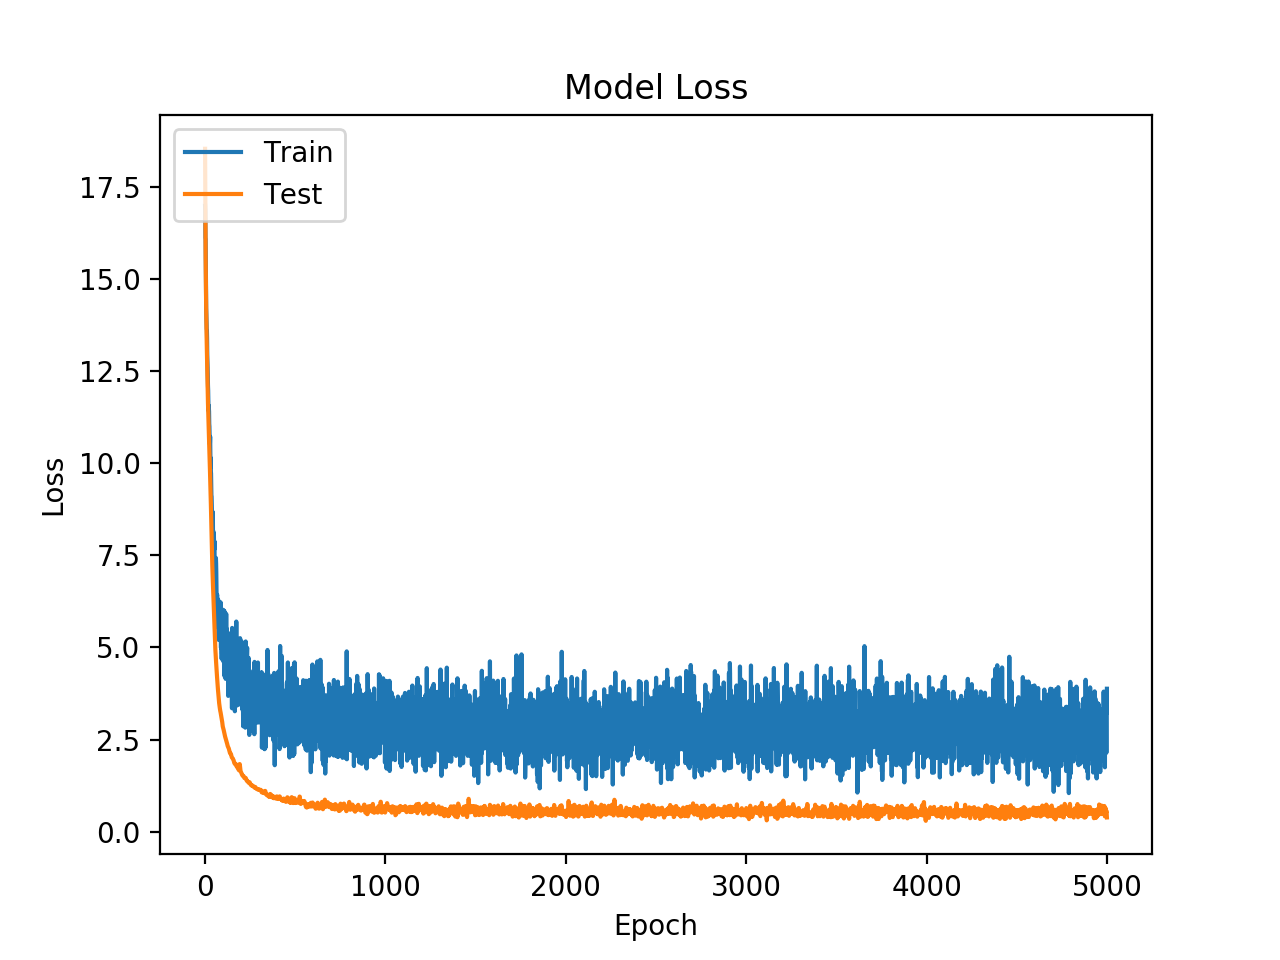
\includegraphics[width=0.8\textwidth]{loss.png}
\caption{}
\end{figure}


\begin{figure}[h] 
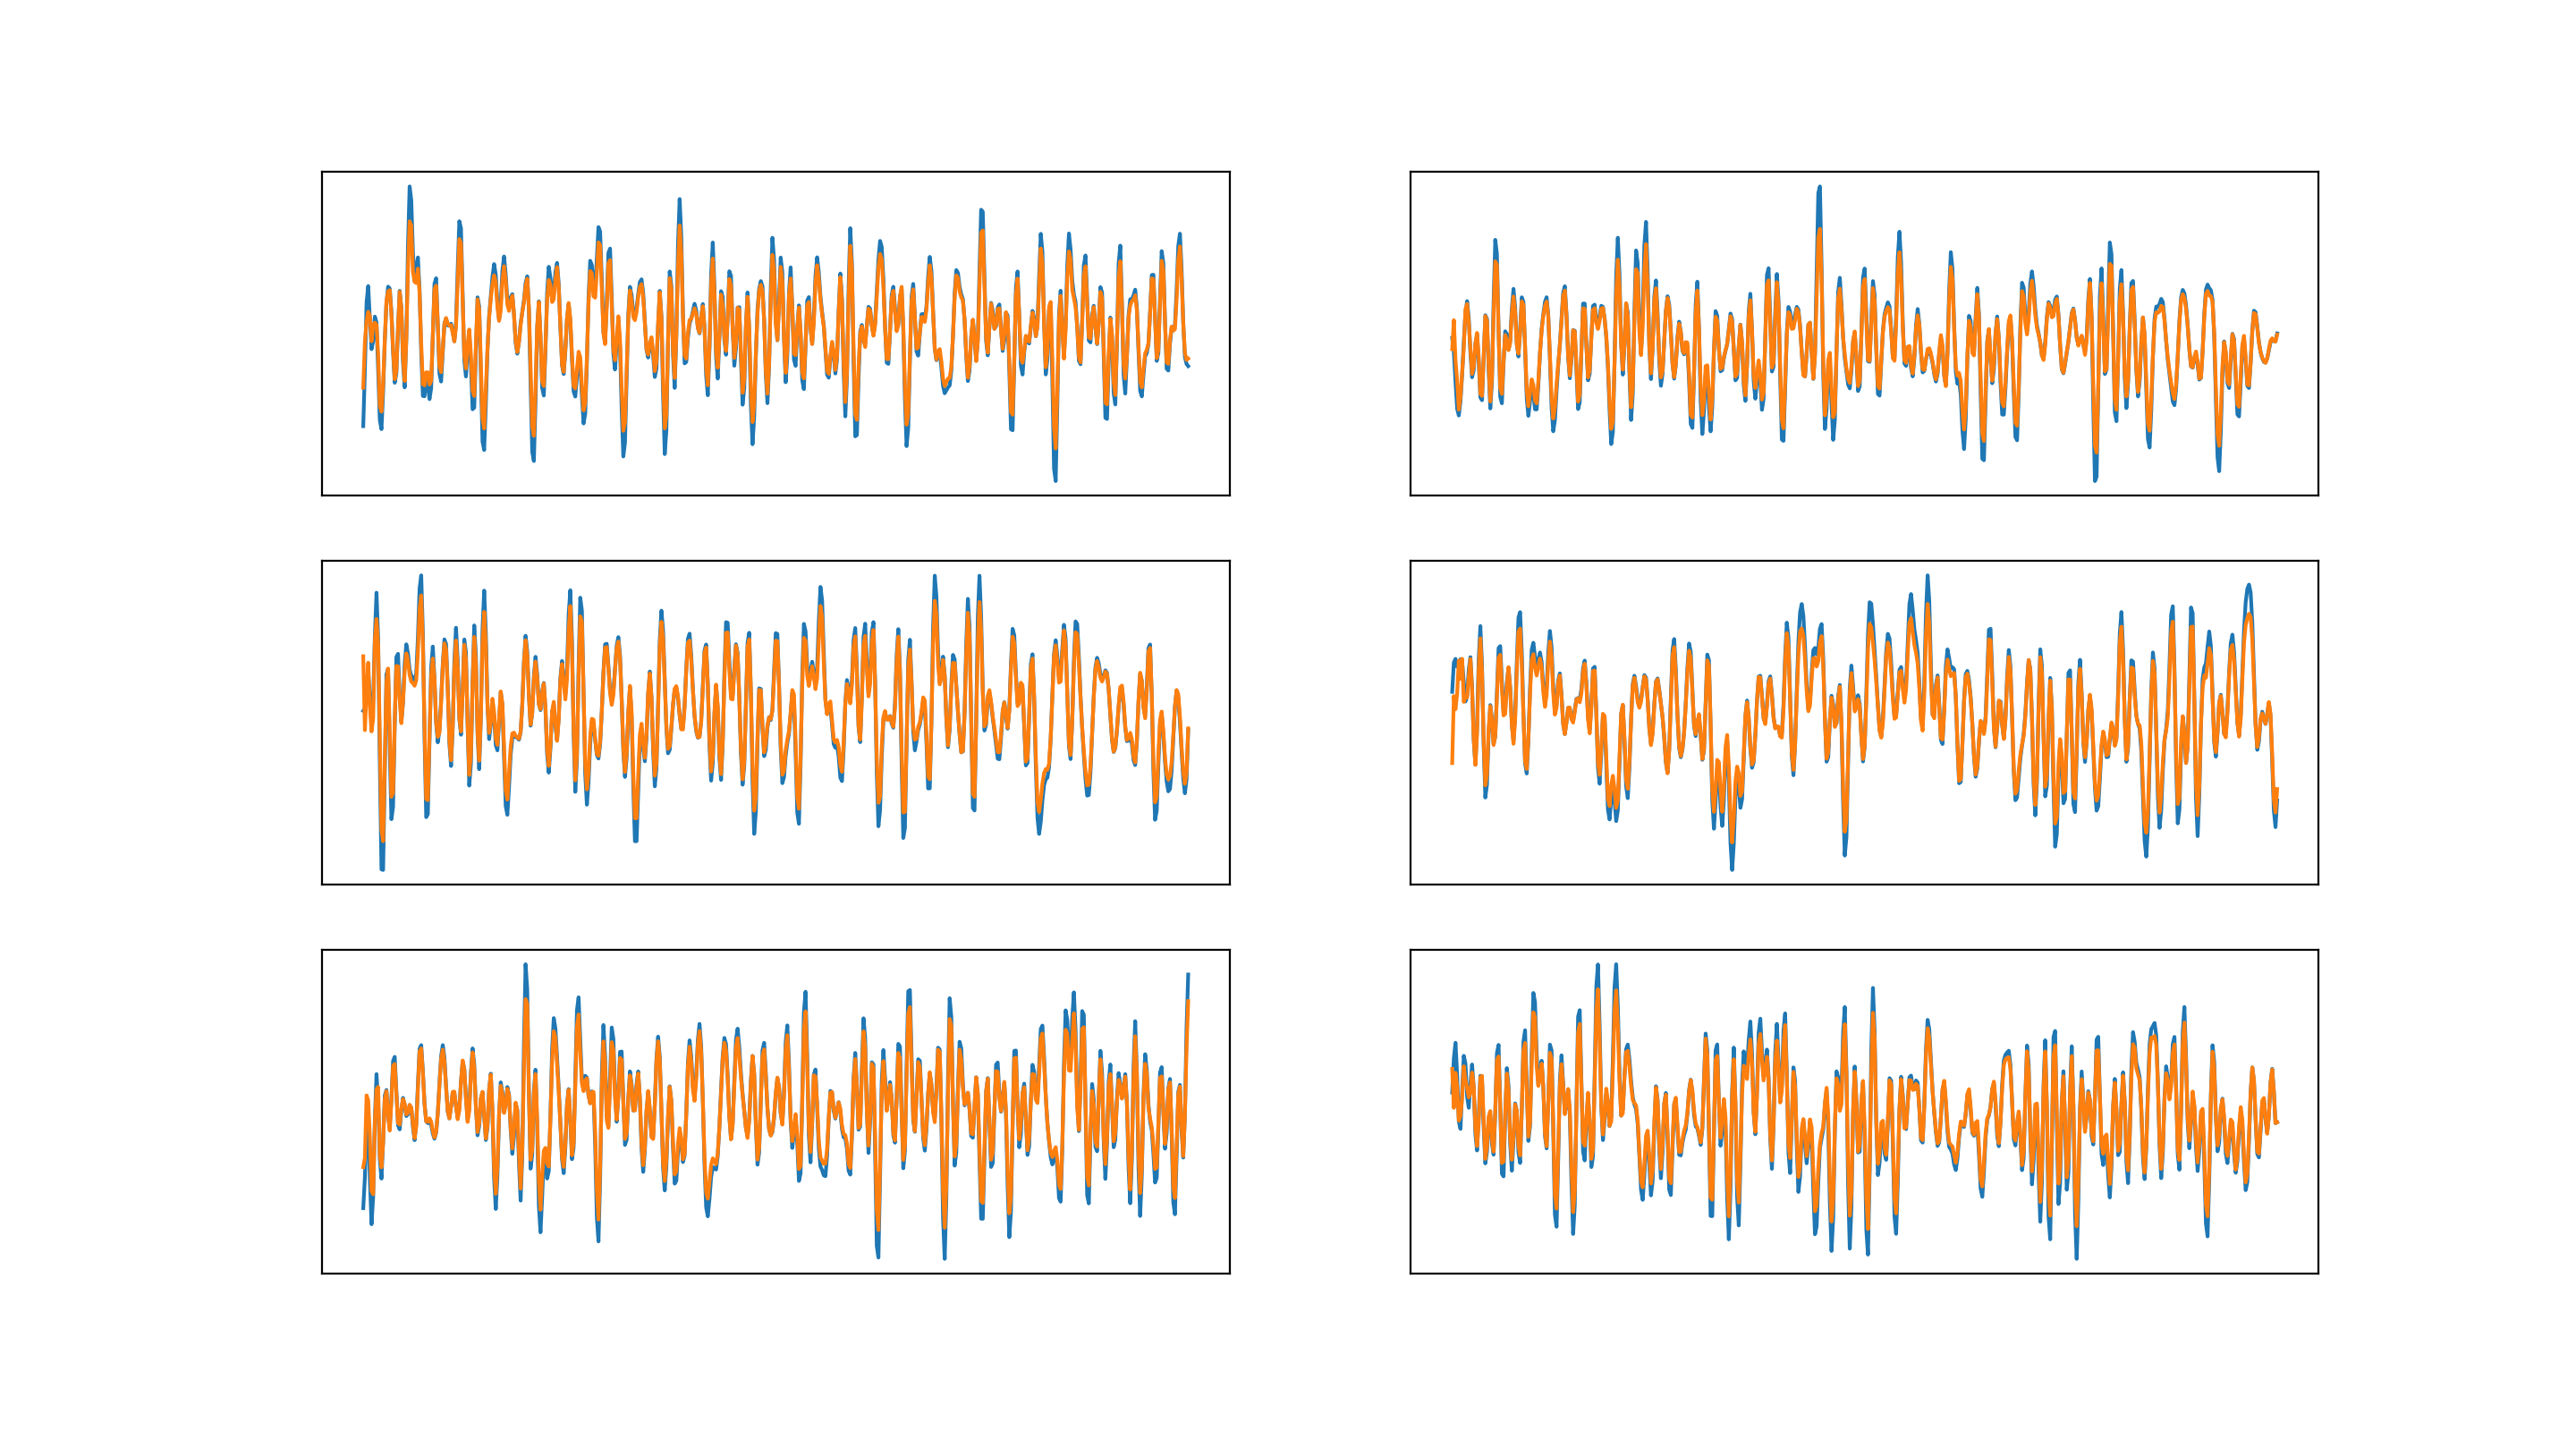
\includegraphics[width=1.05\textwidth]{fit.png}
\caption{}
\end{figure}




\end{document}




